\documentclass[11pt,a4paper]{article}
\usepackage[T1]{fontenc}
\usepackage[utf8]{inputenc}
\usepackage{lmodern}
\usepackage[margin=2.5cm]{geometry}
\usepackage{amsmath,amssymb,bm}
\usepackage{graphicx}
\usepackage{booktabs}
\usepackage{microtype}
\usepackage{caption}
\usepackage[numbers,sort&compress]{natbib}
\usepackage{tikz}
\usetikzlibrary{arrows.meta,positioning,fit,backgrounds}
\usepackage[hidelinks]{hyperref}
\usepackage{xcolor}
\captionsetup{font=small,labelfont=bf}
\graphicspath{{figures/}}
\newcommand{\z}{\bm{z}}
\newcommand{\n}{\bm{n}}
\newcommand{\R}{\mathsf{R}}
\renewcommand{\arraystretch}{1.12}
\newcommand{\doi}[1]{\url{https://doi.org/#1}}

\title{\textbf{Celestial Geolocation from a Single Night-Sky Photograph without a Visible Horizon, using Star-Calibrated Vertical Edges}}
\author{Aaroh Verma\\ {\small University of Illinois Urbana-Champaign, Urbana, IL 61801, USA}\\ {\small\texttt{aarohv2@illinois.edu}}\\ {\small ORCID: \href{https://orcid.org/0009-0007-3763-2895}{0009-0007-3763-2895}}}
\date{}

\begin{document}
\maketitle

\begin{abstract}
\noindent A photograph of the night sky, together with the time it was taken, contains enough information to locate the photographer: the point of the sky directly overhead (the zenith) has declination equal to the observer's latitude and right ascension equal to local sidereal time. Recovering that point from an ordinary photograph needs two things: the identity and geometry of the stars in the frame, and the direction of local vertical. Existing approaches take the vertical from a visible sea or land horizon, or from an inertial sensor. Neither is available in a typical phone photograph taken in a town, where the horizon is hidden by buildings and no sensor data is stored. We present Starfix, a fully automatic pipeline that (i) recognises the star field blindly with a triangle-hash plate solver hardened by a sky mask, a matched filter, a learned point-source classifier and a geometric trail filter; (ii) recovers the local vertical from the edges of buildings and poles, using the star-calibrated camera to treat every truly vertical edge as a great circle through the zenith and rejecting non-vertical edges by a truncated-loss (MSAC) consensus with local refinement; (iii) solves camera, zenith and an unknown terrain elevation of the horizon in one least-squares adjustment, in which atmospheric refraction of low stars provides an independent level reference; and (iv) reports a calibrated uncertainty from a gradient-boosted model trained on the solver's own diagnostics. In 300-photograph simulated ablations, edge consensus reduces the median error from 150\,km to 30\,km when 15\% of edges are not vertical, and from 234\,km to 34\,km at 30\%; the joint terrain adjustment halves the median error behind hills (76\,$\to$\,38\,km) and mountains (188\,$\to$\,99\,km). On 60 rendered photographs the full pipeline recognised every sky, with a median error of 1.3\,km. On one real, uncontrolled phone photograph with no horizon and no metadata, 18 building edges located the photographer 1.6\,km from the true position. To our knowledge, star-calibrated vertical vanishing points from man-made structure have not previously been used for a celestial position fix. The software runs entirely in a web browser and is released with all data and scripts.
\end{abstract}

\noindent\textbf{Keywords:} celestial navigation; astrometry; plate solving; vanishing points; image geolocation; robust estimation; uncertainty calibration

%======================================================================
\section{Introduction}

Celestial navigation determines position from the observed directions of stars relative to the local vertical. With a sextant, the vertical is supplied by the sea horizon; with an automated star tracker it is supplied by an inertial measurement unit or an inclinometer. In either case the astronomy is simple: at a known instant, the zenith direction $\z$ expressed in equatorial coordinates $(\alpha_z,\delta_z)$ gives
\begin{equation}
\varphi = \delta_z, \qquad \lambda = \alpha_z - \theta_{\mathrm{G}}(t),
\label{eq:fix}
\end{equation}
where $\varphi$ is latitude, $\lambda$ east longitude and $\theta_{\mathrm G}$ Greenwich sidereal time at the instant of exposure $t$. The difficulty lies entirely in measuring $\z$.

Night-sky photographs are now taken by billions of phone cameras, and a large fraction show stars above a city street, a house or a campus building. Locating such a photograph is useful for verifying the claimed origin of an image, for recovering the location of historical or field photographs that lack metadata, and as a teaching tool for celestial navigation. Two obstacles stand in the way. First, the star field must be recognised in a noisy, compressed image in which street lights, hot pixels, aircraft trails and lit facades outnumber the stars. Second, a phone photograph rarely shows a clean horizon, and stores no orientation sensor data in the file. Without a vertical reference, the star field fixes the camera's orientation in the sky but not the observer's position on the Earth.

The central observation of this paper is that \emph{the built environment is itself a vertical reference}. Wall corners, window frames, door jambs and lamp posts are constructed plumb to within a few tenths of a degree. In image-based camera calibration, the vanishing point of such edges is a standard cue to camera tilt \citep{zhai2016horizon,pautrat2023deeplsd}. Once the stars have fixed the camera's intrinsic parameters and its orientation in the celestial frame, the vertical vanishing point stops being a property of the camera and becomes a direction in the sky: the zenith. Each vertical edge, back-projected through the calibrated camera, defines a plane through the camera centre that must contain $\z$. Two edges give $\z$; many edges over-determine it and allow non-vertical edges (roof slopes, perspective-distorted facades, branches) to be rejected.

Our contributions are:
\begin{enumerate}\itemsep0pt
\item A method for obtaining the local vertical from man-made edges in a star-calibrated photograph, with a robust consensus that tolerates a substantial share of non-vertical edges (Section~\ref{sec:verticals}).
\item A joint sky--ground adjustment that estimates the unknown elevation of a terrain horizon together with the camera and zenith, using the known refraction of low stars as an independent level (Section~\ref{sec:joint}).
\item A learned uncertainty model that turns the solver's own diagnostics into calibrated error bounds (Section~\ref{sec:uncert}).
\item A complete browser-based implementation, with simulation studies, ablations and a demonstration on a real photograph (Sections~\ref{sec:experiments}--\ref{sec:real}).
\end{enumerate}

%======================================================================
\section{Related work}

\paragraph{Automated celestial navigation.} Star trackers determine attitude from star patterns; to determine \emph{position} they need an independent vertical. Practical systems use an inertial platform or a precision inclinometer. A notable alternative, patented by \citet{rosenwinkel2014patent}, measures the vertical from the differential atmospheric refraction of stars at low elevation. We use refraction as a secondary level constraint in the joint adjustment (Section~\ref{sec:joint}), but our primary new vertical reference is architectural.

\paragraph{Astrometric calibration of images.} Blind astrometric solvers identify star fields from geometric hashes of star asterisms. Recently, \citet{gonzalez2026allsky} calibrated low-cost all-sky (fisheye) cameras automatically, assuming a known site and time; they do not estimate location. Our recogniser is a compact triangle-hash solver with a Poisson significance test, sized to run in a browser with a 230-star catalogue and planets.

\paragraph{Vanishing points and the vertical in computer vision.} Estimating the vertical vanishing point and horizon line from line segments is well studied, with robust hypothesis-and-test schemes \citep{zhai2016horizon} and learned line detectors \citep{pautrat2023deeplsd}. Line segments are commonly extracted with LSD \citep{vongioi2010lsd}. Robust estimation in this setting uses RANSAC variants; we use the MSAC truncated loss \citep{torr2000mlesac} with local optimisation \citep{chum2003lo}. These methods recover the vertical \emph{relative to the camera}; to our knowledge they have not been combined with a star-calibrated camera to recover the vertical in the celestial frame and hence a geographic position.

\paragraph{Image geolocation.} Learned geolocation from image content predicts locations at city to continent scale and fails at night. Astronomical approaches using the Sun, sky polarisation or the Moon are coarse without an accurate vertical.

%======================================================================
\section{Method}
\label{sec:method}

Figure~\ref{fig:pipeline} summarises the pipeline. Its only required inputs are the photograph and the time of exposure with its UTC offset; when present, EXIF metadata supplies time, offset and lens focal length.

\begin{figure}[t]
\centering
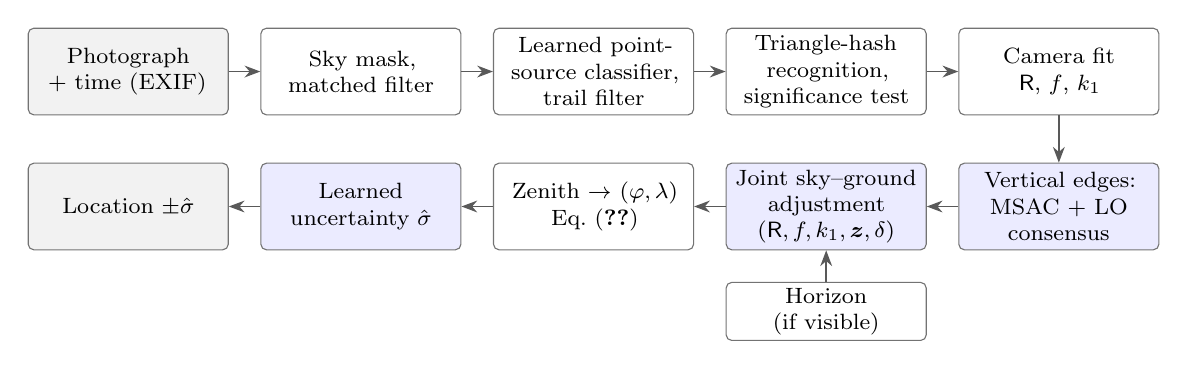
\begin{tikzpicture}[
  box/.style={draw=black!55, rounded corners=2pt, fill=#1, align=center, font=\footnotesize, minimum height=11mm, text width=24mm, inner sep=2pt},
  box/.default=white,
  arr/.style={-{Stealth[length=2mm]}, draw=black!65, line width=0.6pt},
  node distance=6mm and 4mm]
\node[box=black!5] (img) {Photograph\\ + time (EXIF)};
\node[box, right=of img] (mask) {Sky mask,\\ matched filter};
\node[box, right=of mask] (mlp) {Learned point-\\source classifier,\\ trail filter};
\node[box, right=of mlp] (rec) {Triangle-hash\\ recognition,\\ significance test};
\node[box, right=of rec] (cam) {Camera fit\\ $\R$, $f$, $k_1$};
\node[box=blue!8, below=of cam] (vert) {Vertical edges:\\ MSAC + LO\\ consensus};
\node[box=blue!8, left=of vert] (joint) {Joint sky--ground\\ adjustment\\ $(\R,f,k_1,\z,\delta)$};
\node[box, left=of joint] (fix) {Zenith $\to(\varphi,\lambda)$\\ Eq.~\eqref{eq:fix}};
\node[box=blue!8, left=of fix] (gbt) {Learned\\ uncertainty $\hat\sigma$};
\node[box=black!5, left=of gbt] (out) {Location $\pm\hat\sigma$};
\node[box, below=4mm of joint, minimum height=7mm] (hor) {Horizon (if visible)};
\draw[arr] (img) -- (mask); \draw[arr] (mask) -- (mlp); \draw[arr] (mlp) -- (rec); \draw[arr] (rec) -- (cam);
\draw[arr] (cam) -- (vert); \draw[arr] (vert) -- (joint); \draw[arr] (hor) -- (joint);
\draw[arr] (joint) -- (fix); \draw[arr] (fix) -- (gbt); \draw[arr] (gbt) -- (out);
\end{tikzpicture}
\caption{The Starfix pipeline. Shaded blue boxes are the components evaluated by ablation in this paper. When no vertical reference is found, coarse fallbacks (EXIF GPS, the Moon, a rough region) are used instead.}
\label{fig:pipeline}
\end{figure}

\subsection{Finding stars in a photograph of a town}

Phone photographs taken in towns contain far more bright, compact features on the ground than stars in the sky. We therefore first compute a \emph{sky mask} on $4\times4$ pixel cells: each cell's minimum (which ignores stars) and its standard deviation (texture) are box-smoothed, cells that are both dark and smooth relative to the 30th percentile of the image are marked as sky, the mask is cleaned by a morphological opening, and only large connected regions are kept. Candidates are then found as local maxima of the image convolved with a $3\times3$ binomial kernel, a matched filter for a near-Gaussian point spread function, that exceed a robust $5\sigma$ threshold above a $25\times25$ local background; centroids are measured to about 0.1\,pixel by thresholded first moments.

Each candidate is classified by a multilayer perceptron (two hidden layers of 128 and 64 units) on 129 features: an $11\times11$ background-subtracted, peak-normalised patch and eight shape descriptors (second moments, ellipticity, sharpness, peak-to-flux ratio, local contrast). The network is trained on 300{,}000 rendered patches, half stars with Gaussian, Moffat, elongated, defocused and saturated profiles at signal-to-noise ratios from 3 to 400, and half impostors: hot pixels with demosaicing spread, heavy-tailed noise spikes, ground lights with flare, aircraft and satellite trails (including blinking dashes) and bright foreground edges; 65\% of patches are passed through JPEG compression. Finally, a geometric trail filter removes any set of eight or more candidates lying within 1.5\,pixels of a common line, which removes the fragments into which a trail breaks.

\subsection{Recognising the star field}

We index all triangles formed by the brightest catalogue stars (230 stars to magnitude $\approx 2.9$, plus the five naked-eye planets computed with Astronomy Engine \citep{cross2023astronomy}) by their two side ratios. Triangles of bright detections are looked up in this index; each match proposes a camera rotation by Horn's closed-form quaternion solution \citep{horn1987closed} and a focal length. The proposal is scored by predicting every catalogue star into the image and counting detections within a tolerance. Because a busy field matches many stars by chance, a count $k$ is converted to a significance $S = -\log_{10} P(X\ge k)$ with $X\sim\mathrm{Poisson}(\mu)$, where $\mu$ is the number of chance matches expected given the density of detections and the search radius. Proposals with refined $S\ge25$ are accepted immediately; otherwise the best proposal above a lower threshold is accepted after a fixed time budget. When EXIF provides the 35\,mm-equivalent focal length, the search is restricted to it; otherwise a geometric grid of focal lengths covering diagonal fields of view from $12^\circ$ to $140^\circ$ is tried, starting from a typical phone camera.

\subsection{Camera model}

A star with unit direction $\bm{s}$ in the celestial frame, corrected for precession (IAU 1976 \citep{lieske1977}), annual aberration and refraction, is projected as
\begin{equation}
\bm{u} = \R\,\bm{s},\quad
\begin{pmatrix}x\\y\end{pmatrix} = \begin{pmatrix}c_x\\c_y\end{pmatrix} + f\,(1+k_1 \rho^2)\begin{pmatrix}u_1/u_3\\u_2/u_3\end{pmatrix},\quad \rho^2=\frac{u_1^2+u_2^2}{u_3^2},
\end{equation}
with rotation $\R$, focal length $f$, principal point $(c_x,c_y)$ at the image centre and radial distortion $k_1$ (fitted only when seven or more stars are identified). All parameters are refined by Levenberg--Marquardt on pixel residuals, with outlier rejection and progressive admission of fainter catalogue stars. We denote by $\bm{r}(x,y)$ the inverse projection: the unit ray in the celestial frame through pixel $(x,y)$.

\subsection{The vertical from building edges}
\label{sec:verticals}

Let an image segment have endpoints $\bm{p}_1,\bm{p}_2$. Its back-projected rays $\bm{r}_1=\bm{r}(\bm{p}_1)$, $\bm{r}_2=\bm{r}(\bm{p}_2)$ span a plane through the camera centre with unit normal $\n=(\bm{r}_1\times\bm{r}_2)/\|\bm{r}_1\times\bm{r}_2\|$. If the segment images a vertical line in the world, that plane contains the local vertical, so
\begin{equation}
\z\cdot\n = 0 .
\label{eq:edge}
\end{equation}
Since $\R$ and $f$ are known from the stars, Eq.~\eqref{eq:edge} is a constraint on $\z$ \emph{directly in the celestial frame}. The residual of edge $i$ is $e_i = \z\cdot\n_i$, with standard deviation
\begin{equation}
\sigma_i = \sqrt{\left(\frac{\sqrt2\,\sigma_{\mathrm{px}}}{f\,\theta_i}\right)^2 + \sigma_{\mathrm{lean}}^2},
\label{eq:edgesig}
\end{equation}
where $\theta_i$ is the angular length of the segment, $\sigma_{\mathrm{px}}$ the endpoint uncertainty and $\sigma_{\mathrm{lean}}=0.3^\circ$ the typical deviation of a constructed ``vertical'' from true plumb. Long, well-measured edges therefore constrain $\z$ tightly, and the lean term prevents any single edge from dominating.

\paragraph{Candidate edges.} Up to 80 of the longest segments in the ground (non-sky) region are extracted with an LSD-style region-growing detector \citep{vongioi2010lsd}, with a minimum length of 2.2\% of the image diagonal. An automatic finder then forms a zenith hypothesis $\z\propto\n_i\times\n_j$ from every pair of segments and keeps only hypotheses that are physically admissible: every identified star must be more than $1^\circ$ above the horizon defined by $\z$, and the vertical must appear within $55^\circ$ of image-upright. Each admissible hypothesis is scored by the length-weighted number of segments that satisfy Eq.~\eqref{eq:edge} within $0.5^\circ$--$1^\circ$; segments whose direction lies within $20^\circ$ of the hypothesised zenith are ignored, since edges pointing almost at the zenith (often roof overhangs seen from below) constrain it poorly. The best hypothesis must be supported by at least three segments, and its supporters become the candidate edges. The user may also trace edges by hand.

\paragraph{Consensus.} Many candidate edges are not vertical: sloping roofs, gutters seen in perspective, tree trunks, cables. We estimate $\z$ robustly in three stages. (1) If the least-squares solution using all edges leaves every edge within its tolerance $\tau_i = \min(1.5^\circ,\max(0.6^\circ,3\sigma_i))$, all are kept. (2) Otherwise, every pair of non-parallel edges $(i,j)$ proposes $\z_{ij} \propto \n_i\times\n_j$ (sign chosen towards the stars), which is scored by the MSAC cost \citep{torr2000mlesac}
\begin{equation}
C(\z) = \sum_k \min\!\left(\frac{(\z\cdot\n_k)^2}{\sigma_k^2},\; 9\right).
\end{equation}
Exhaustive enumeration is affordable because the number of candidate edges is modest (tens). (3) The best hypothesis is refined by local optimisation \citep{chum2003lo}: refit $\z$ to its inliers, re-admit every edge within tolerance, and iterate to convergence.

\subsection{Joint sky--ground adjustment}
\label{sec:joint}

Where a horizon is visible, its points $\bm{h}_j$ satisfy $\z\cdot\bm{r}(\bm{h}_j) = \sin(a_0+\delta)$, where $a_0$ is the expected apparent altitude of the horizon (zero for a sea horizon before dip) and $\delta$ the unknown elevation angle of distant terrain. Assuming $\delta=0$ for a hilly horizon biases $\z$ by the full terrain elevation. We instead estimate the parameter vector $(\R,f,k_1,\z,\delta)$ jointly by minimising
\begin{multline}
\chi^2 = \sum_{\text{stars}} \frac{\|\bm{x}_s - \pi(\R,f,k_1;\, \mathcal{A}(\bm{s},\z))\|^2}{\sigma_{\mathrm{px}}^2 + (0.1\,f\,\Delta_{\mathrm R}(a_s))^2}
+ \sum_{\text{horizon}} \frac{\left(\z\cdot\bm{r}(\bm{h}_j) - \sin(a_0+\delta)\right)^2}{\sigma_h^2} \\
+ \sum_{\text{edges}} \frac{(\z\cdot\n_i)^2}{\sigma_i^2}
+ \frac{\delta^2}{\sigma_{\mathrm{terr}}^2},
\label{eq:joint}
\end{multline}
where $\mathcal{A}(\bm{s},\z)$ applies refraction towards the zenith $\z$, with refraction at apparent altitude $a$ (degrees)
\begin{equation}
\Delta_{\mathrm R}(a) = \frac{1.02'}{\tan\left(a + 10.3/(a+5.11)\right)}
\end{equation}
 \citep{saemundsson1986,bennett1982}, assigned a 10\% model uncertainty. The terrain prior $\sigma_{\mathrm{terr}}$ depends on the horizon type selected (sea, flat, buildings, trees, hills, mountains). The key point is that refraction couples the star positions to $\z$: low stars are lifted by up to $0.5^\circ$, and the pattern of this lift across the field fixes a level reference independent of the terrain. The horizon then mainly constrains the \emph{direction} of tilt, while the elevation offset $\delta$ is absorbed. The adjustment is solved by Gauss--Newton with numerical Jacobians; its covariance is propagated to north--south and east--west errors in kilometres.

\subsection{Calibrated uncertainty}
\label{sec:uncert}

The formal covariance of Eq.~\eqref{eq:joint} ignores model errors (terrain mis-specification, misidentified edges, clock error) and is poorly calibrated. We therefore train two gradient-boosted regression ensembles \citep{friedman2001gbm} (400 trees, Huber loss) to predict $\log|e_{\mathrm{NS}}|$ and $\log|e_{\mathrm{EW}}|$ from 20 solver diagnostics: the log formal standard deviations in each direction, the numbers of stars, horizon points and edges, the angular span of the horizon, the fitted terrain offset $|\delta|$ and its standard deviation, the share of low-altitude stars, the residual RMS, the field of view, the camera altitude, $|\varphi|$, the log of the declared clock uncertainty, and the horizon type (one-hot). For a zero-mean Gaussian error, $\mathbb{E}\log|e| = \log\sigma - (\gamma+\log 2)/2$ with $\gamma$ Euler's constant, so the prediction is converted to $\hat\sigma = s\,\exp\!\big(\hat g(\bm{x}) + (\gamma+\log2)/2\big)$, and a single scale $s$ is set on a calibration split so that a target share of fixes falls within $2\hat\sigma$. Clock error enters longitude directly: one second of time is $15''$ of longitude, or $0.46\cos\varphi$\,km.

\subsection{Fallbacks}

When no vertical can be found, Starfix returns, in order of preference: GPS coordinates from EXIF if present; a circle of position from the Moon's measured altitude; or a coarse probability map combining the constraints that every star is above the horizon, the camera roll is near upright (prior $\sigma=30^\circ$), longitude is consistent with the time-zone offset ($\sigma=10^\circ$), and a population prior. These fallbacks are not evaluated here.

%======================================================================
\section{Experiments}
\label{sec:experiments}

No public dataset of night-sky photographs with ground-truth location and a recorded vertical reference exists. We therefore evaluate on simulations built with real star positions, realistic camera models and noise, and report one real photograph separately (Section~\ref{sec:real}). All experiments use the same JavaScript code as the public web application; scripts and outputs are in the released repository. Medians are reported with 95\% bootstrap confidence intervals (4{,}000 resamples); paired comparisons use the Wilcoxon signed-rank test; proportions use Wilson intervals.

\paragraph{Simulation.} Each simulated photograph draws a location uniformly over the sphere between latitudes $-60^\circ$ and $+72^\circ$, a random instant in 2020--2031, and a camera of 35\,mm-equivalent focal length 13--35\,mm (4:3 or 3:2, radial distortion $k_1$ up to 0.08) with roll $\mathcal N(0,3^\circ)$. Refraction is applied with a random scale error of 8\% (1$\sigma$); centroid noise is 0.25--2.5\,pixels; 0--40\% of visible stars are dropped and 6--40 of the brightest are kept. In 70\% of trials the vertical reference is a horizon of one of six types, with terrain elevation drawn per type (sea: dip for heights of 0.5--60\,m; flat: $|\mathcal N(0,0.08^\circ)|$; hills: $0.1^\circ$--$1.2^\circ$; trees and rooflines: $0.2^\circ$--$2.5^\circ$; mountains: $0.4^\circ$--$3.5^\circ$), plus local roughness, and the camera points low enough to include it. In the remaining 30\% the camera points $10^\circ$--$80^\circ$ up and the reference is a set of vertical edges: either 3--20 found automatically (endpoint noise 0.7\,pixel) or 2--4 traced by hand (1.2\,pixel), each leaning by $\mathcal N(0,0.3^\circ)$, with 15\% replaced by non-vertical distractors tilted $2^\circ$--$10^\circ$. The clock error is Gaussian with standard deviation half of a declared accuracy of 2\,s, 30\,s, 2\,min, 10\,min or 1\,h.

\subsection{Recognition}

Two hundred simulated star fields (five lenses, with and without EXIF focal length, 20 each) were rendered as detection lists including spurious detections. Table~\ref{tab:recognition} shows that phone-camera fields of view are recognised almost always; failure at longer focal lengths is explained by the small catalogue (Fig.~\ref{fig:recognition}): recognition is reliable with 13 or more catalogue stars in the frame and impossible with five or fewer. Across the 146 recognised fields, 9 of 2{,}914 star identifications (0.3\%) were wrong; the median focal-length error was 0.06\%.

\begin{table}[t]
\centering\footnotesize
\caption{Recognition rate by lens (20 simulated fields per cell; 95\% Wilson interval in brackets) and median time per field on a laptop browser.}
\label{tab:recognition}
\begin{tabular}{lcccc}
\toprule
Lens (35\,mm eq.) & Catalogue stars & With EXIF $f$ & Without & Time (with / without) \\
\midrule
13\,mm (ultra-wide) & 33 & 100\% [84, 100] & 95\% [76, 99] & 0.4\,s / 9.8\,s \\
24\,mm & 18 & 90\% [70, 97] & 85\% [64, 95] & 0.6\,s / 2.8\,s \\
26\,mm (phone main) & 17 & 100\% [84, 100] & 100\% [84, 100] & 0.5\,s / 1.1\,s \\
35\,mm & 8 & 55\% [34, 74] & 50\% [30, 70] & 11.6\,s / 10.8\,s \\
50\,mm & 5 & 35\% [18, 57] & 20\% [8, 42] & 11.5\,s / 11.8\,s \\
\bottomrule
\end{tabular}
\end{table}

\begin{figure}[t]
\centering
\begin{minipage}[t]{0.47\textwidth}\centering
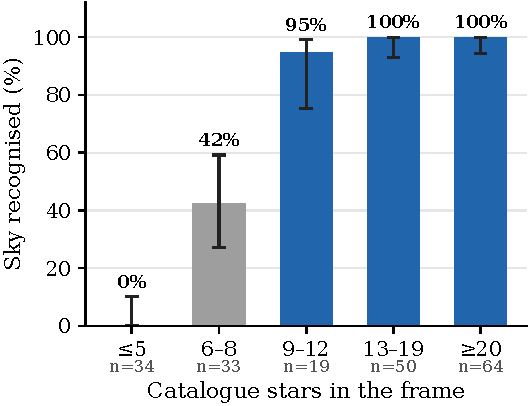
\includegraphics[width=\linewidth]{fig_recognition.pdf}
\caption{Recognition rate against the number of catalogue stars in the frame, pooled over lenses (Wilson 95\% intervals).}
\label{fig:recognition}
\end{minipage}\hfill
\begin{minipage}[t]{0.49\textwidth}\centering
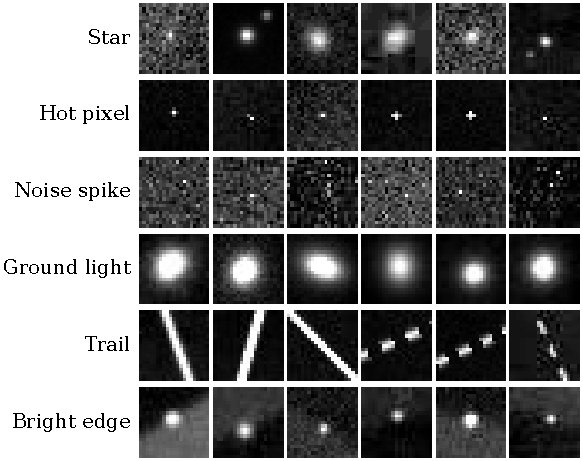
\includegraphics[width=0.92\linewidth]{fig_patches.pdf}
\caption{Examples of rendered training patches for the point-source classifier, one class per row.}
\label{fig:patches}
\end{minipage}
\end{figure}

\subsection{Point-source classifier and the full pipeline}

On 60{,}000 held-out rendered patches (Fig.~\ref{fig:patches}), the classifier reaches 96.5\% accuracy (ROC AUC 0.995), keeping 96.3\% of stars while rejecting 96.9\% of hot pixels, 99.4\% of noise spikes, 94.3\% of ground lights, 97.1\% of trail fragments and 98.2\% of bright edges.

To test detection and recognition together, we rendered 60 full-resolution phone photographs (26\,mm equivalent, flat horizon, exact clock) with 0--400 hot pixels, 0--3 satellite trails, sky glow, sensor noise and JPEG compression, and ran the complete pipeline on the images. With the classifier, all 60 skies were recognised (Wilson 95\% interval 94--100\%) and 56 produced a fix, with median error 1.3\,km (95\% CI 1.0--1.6\,km) and 90th percentile 3.5\,km. With the classifier disabled, only 22 of 60 were recognised (26--49\%). These rendered scenes have a perfectly flat, cleanly detected horizon and no terrain or atmospheric model error; they measure the image-processing chain, not the end-to-end accuracy, which is the subject of the next section.

\subsection{Ablation: edge consensus and joint terrain adjustment}

Each ablation uses 300 simulated photographs per condition and evaluates the solver with and without one component on identical inputs (Fig.~\ref{fig:ablations}, Table~\ref{tab:ablations}).

\emph{Edge consensus.} With all edges truly vertical, consensus changes nothing (median 27\,km both ways), confirming that the all-edge check prevents needless discarding of good edges. When 15\% of edges are not vertical, using every edge raises the median error to 150\,km, whereas consensus keeps it at 30\,km; at 30\% the figures are 234\,km and 34\,km. The 90th percentile falls from 491 to 73\,km and from 744 to 106\,km respectively.

\emph{Joint terrain adjustment.} On flat horizons there is no difference (10.8 vs.\ 10.9\,km; $p=0.17$). Behind hills, estimating $\delta$ halves the median error from 76 to 38\,km and improves 79\% of photographs; behind mountains it falls from 188 to 99\,km, improving 76\%.

\begin{figure}[t]
\centering
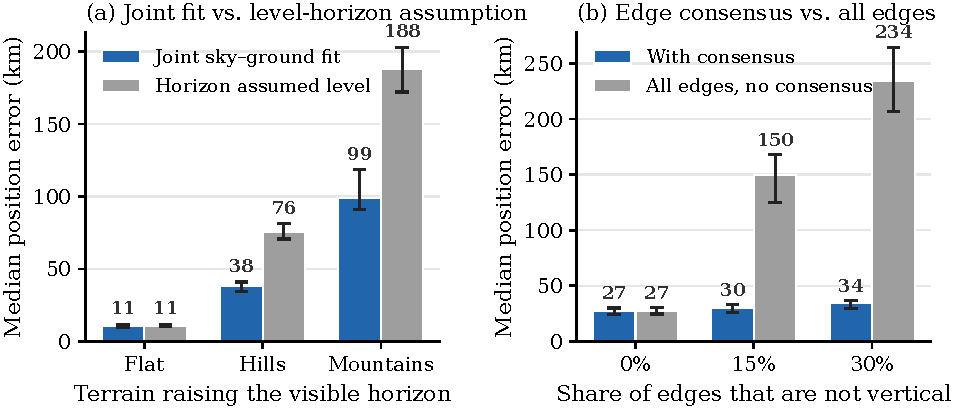
\includegraphics[width=\textwidth]{fig_ablations.pdf}
\caption{Ablations on 300 simulated photographs per group (median and 95\% bootstrap interval). (a) Estimating the terrain elevation jointly with the zenith versus assuming a level horizon. (b) Consensus over vertical edges versus a least-squares fit to all candidate edges.}
\label{fig:ablations}
\end{figure}

\begin{table}[t]
\centering\small
\caption{Ablation results (300 photographs per row). Medians with 95\% bootstrap intervals; ``better'' is the share of photographs whose error the component reduced; $p$ from a paired Wilcoxon signed-rank test.}
\label{tab:ablations}
\begin{tabular}{llcccc}
\toprule
Component & Condition & With (km) & Without (km) & Better & $p$ \\
\midrule
Joint terrain fit & Flat & 10.8 [9.9, 11.7] & 10.9 [10.2, 11.7] & 46\% & 0.17 \\
 & Hills & 38.5 [34.6, 41.0] & 75.8 [70.6, 81.0] & 79\% & $10^{-29}$ \\
 & Mountains & 98.7 [90.9, 119.1] & 187.9 [172.1, 203.1] & 76\% & $10^{-16}$ \\
\midrule
Edge consensus & 0\% non-vertical & 27.0 [24.1, 30.1] & 27.0 [24.3, 30.1] & -- & -- \\
 & 15\% non-vertical & 29.9 [25.8, 33.1] & 149.6 [125.3, 168.3] & 76\% & $10^{-38}$ \\
 & 30\% non-vertical & 34.5 [30.0, 37.0] & 234.1 [206.6, 265.1] & 90\% & $10^{-36}$ \\
\bottomrule
\end{tabular}
\end{table}

\subsection{End-to-end accuracy}

Over 40{,}000 simulated photographs, the source of the vertical dominates the error (Fig.~\ref{fig:cdf}, Table~\ref{tab:source}). With a clock accurate to 2\,s, a sea horizon gives a median of 11\,km and a flat land horizon 13\,km. Vertical edges alone give a median of 44\,km; their distribution has a heavy tail (90th percentile 650\,km) from photographs with only two or three short, nearly parallel edges, which constrain $\z$ only in one direction. Clock error adds directly to longitude: the median over all photographs is 43\,km with a 2\,s clock, 52\,km at 2\,min, 114\,km at 10\,min and 471\,km at 1\,h.

\begin{figure}[t]
\centering
\begin{minipage}[b]{0.56\textwidth}\centering
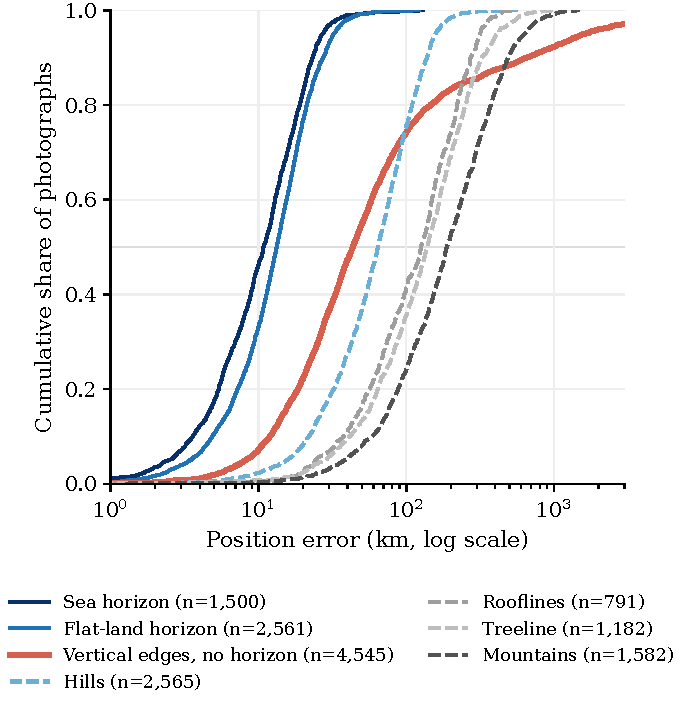
\includegraphics[width=\linewidth]{fig_error_cdf.pdf}
\caption{Cumulative distribution of position error by source of the vertical (40{,}000 simulated photographs; clock exact to 2\,s).}
\label{fig:cdf}
\end{minipage}\hfill
\begin{minipage}[b]{0.41\textwidth}\centering\small
\captionof{table}{Error by source of the vertical (km; clock 2\,s).}
\label{tab:source}
\begin{tabular}{lrrr}
\toprule
Source & $n$ & Median & P90 \\
\midrule
Sea & 1500 & 10.8 & 23 \\
Flat land & 2561 & 13.3 & 27 \\
Edges only & 4545 & 43.6 & 650 \\
Hills & 2565 & 64.5 & 138 \\
Rooflines & 791 & 126.2 & 273 \\
Treeline & 1182 & 137.9 & 323 \\
Mountains & 1582 & 188.0 & 488 \\
\bottomrule
\end{tabular}
\vspace{6mm}
\end{minipage}
\end{figure}

\subsection{Calibration of the reported uncertainty}

The learned model was trained on 27{,}200 photographs, calibrated on 4{,}800 and tested on 8{,}000 held-out photographs. Figure~\ref{fig:calibration} compares the share of true positions inside $\pm k\hat\sigma$ with the ideal Gaussian curve, for the learned $\hat\sigma$ and for the formal covariance scaled by a hand-tuned factor. At $2\hat\sigma$ the learned model covers 93.2\% (north--south) and 93.4\% (east--west) of photographs, against 90.7\% and 93.5\% for the scaled formal covariance. More importantly for a user, the learned $\hat\sigma$ ranks good and bad fixes better: the Spearman correlation between $\hat\sigma$ and the actual error is 0.75 versus 0.70 (north--south) and 0.76 versus 0.72 (east--west).

\begin{figure}[t]
\centering
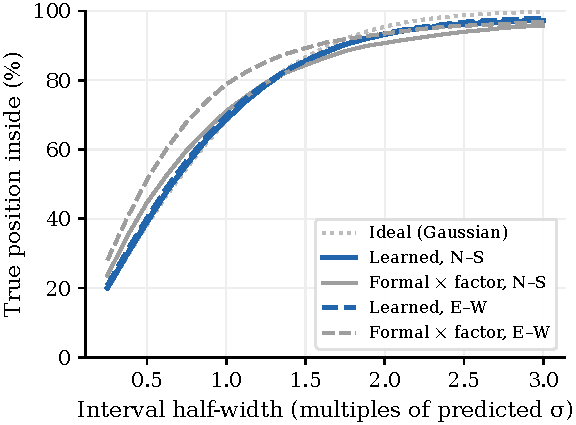
\includegraphics[width=0.62\textwidth]{fig_calibration.pdf}
\caption{Coverage of the reported uncertainty on 8{,}000 held-out simulated photographs.}
\label{fig:calibration}
\end{figure}

%======================================================================
\section{A real photograph}
\label{sec:real}

Figure~\ref{fig:real} shows an uncontrolled phone photograph taken at 01:01 local time (UTC$-6$) on 12 November 2026 in Champaign, Illinois, USA, pointing about $59^\circ$ up past a lit building. The file has no EXIF metadata (no time, lens or orientation), there is no visible horizon, and the lit facade and windows produce many bright spurious features. The time and UTC offset were entered by hand.

The detector found 747 candidates; the classifier kept 469 and the trail filter removed 173 fragments. Sixteen stars in Taurus, Orion, Gemini, Perseus, Auriga and Canis Minor were identified, giving a fitted focal length of 28.4\,mm equivalent, $k_1=0.024$, and an RMS residual of $1.9'$. Of 80 segments examined, 18 building edges supported the best zenith hypothesis, and all 18 were retained by consensus. Their back-projected planes converge on a zenith that lies just above the frame, 0.5\,pixel from the true zenith computed from the known location. The resulting fix is 1.6\,km from the true position, with a learned $1\sigma$ uncertainty of 64\,km (north--south) and 32\,km (east--west). Using all 20 near-vertical segments without consensus gave an error of 488\,km; without the sky mask or without the classifier, recognition still succeeded but with fewer stars (13 and 14), and with neither it failed.

An error of 1.6\,km is far smaller than the stated uncertainty, and a single photograph cannot establish accuracy; the simulation results above are the appropriate expectation for edge-only fixes. The example does show that every stage of the method operates on a real, unprepared image.

\begin{figure}[t]
\centering
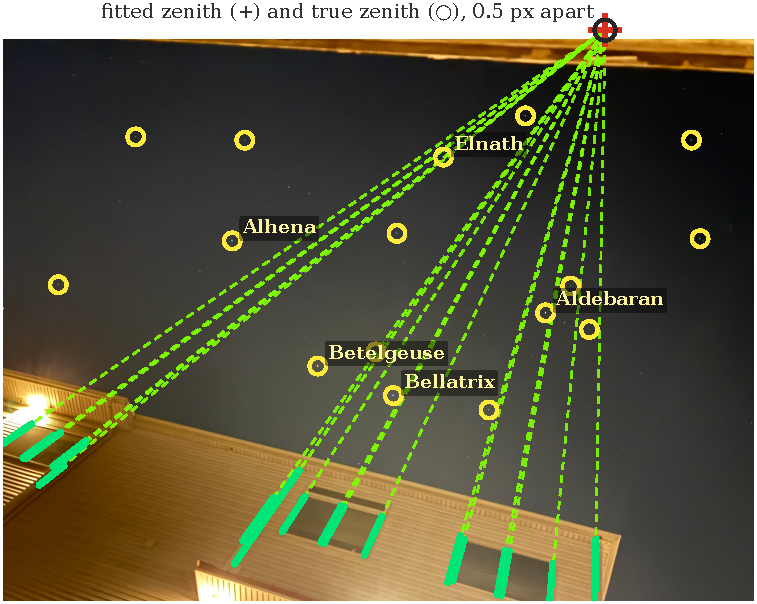
\includegraphics[width=\textwidth]{fig_realphoto.pdf}
\caption{Real phone photograph, Champaign, Illinois, 12 November 2026, 07:01 UTC, no EXIF data. Yellow circles: the 16 identified stars (brightest labelled). Solid green: the 18 vertical edges retained by consensus; dashed: their extensions, which meet at the fitted zenith (+) above the frame, 0.5\,pixel from the true zenith ($\circ$).}
\label{fig:real}
\end{figure}

%======================================================================
\section{Discussion and limitations}

\paragraph{Evaluation on real data.} The principal limitation of this study is that it rests on simulation and a single real photograph. The simulations use real star positions, measured camera models, realistic noise and a refraction model with random error, but the terrain and edge-lean distributions are assumptions. A benchmark of real photographs with known location and time, covering lenses, terrain and building types, is the most important next step and will be released with a future version.

\paragraph{When the method fails.} Narrow lenses (35\,mm and above) often contain too few of the 230 catalogue stars for recognition; a deeper catalogue would remove this limit at a cost in index size. Edges must be truly plumb and reasonably long; scenes dominated by trees or by one short edge give weak or biased verticals, and two near-parallel edges constrain the zenith in only one direction, which produces the heavy tail of Table~\ref{tab:source}. Longitude is only as good as the clock: four minutes of time error is one degree of longitude.

\paragraph{Privacy and misuse.} The method locates a photograph without any metadata, and therefore could be used to locate people who share night-sky photographs. Its accuracy from edges alone (tens of kilometres typically) is at town-to-region scale, and the time of exposure must be known, but users and platforms should be aware of the capability.

\paragraph{Novelty.} Each ingredient (plate solving, vanishing-point estimation, robust consensus, refraction-based levelling, gradient boosting) is established. To our knowledge, the combination proposed here, in which a star-calibrated camera turns the vertical vanishing point of man-made structure into a celestial zenith and hence a geographic fix, has not been described before. Prior position-from-stars systems obtain the vertical from a horizon, inertial sensors, inclinometers or differential refraction \citep{rosenwinkel2014patent}; prior vertical-from-lines work recovers the vertical relative to the camera, not in the celestial frame.

%======================================================================
\section{Conclusion}

Starfix locates a night-sky photograph from the image and its time alone, including when no horizon is visible, by treating the building edges in the photograph as plumb lines calibrated against the stars. Consensus over edges and joint estimation of the terrain horizon each remove most of the error that a naive solution incurs, and a learned model reports how far each fix can be trusted. The implementation runs in an ordinary web browser with no server, and all code, models, data and experiment scripts are released.

\section*{Data and code availability}
The web application, trained models, Python training code, simulation data (40{,}000 photographs) and every experiment script and result reported here are available at \url{https://github.com/Aaroh-Mystogan/starfix} and will be archived with a DOI on Zenodo on acceptance. The real photograph in Fig.~\ref{fig:real} was taken by the author.

\section*{Use of AI tools}
The research question, the overall approach and the workflow of this study were conceived by the author: locating a night-sky photograph from its stars and capture time, using the image content itself rather than metadata, and testing the method on simulations and a real photograph taken by the author. A large language model (Claude, Anthropic) was used extensively as an assistant throughout the project. Specifically, it was used to (i) write and debug substantial parts of the software, including the plate solver, the edge-consensus and joint-adjustment code and the model-training scripts; (ii) propose and refine algorithmic components under the author's direction; (iii) design and run the simulation experiments and produce the figures; (iv) search and summarise the literature and verify references; and (v) draft and edit the text of this manuscript. The author defined the goals, made the decisions about which methods to pursue, supplied the real test photograph and its ground truth, reviewed the code, results and text, and takes full responsibility for the content of this article. The AI tool is not an author.

\section*{Competing interests}
The author declares no competing interests.

\begin{thebibliography}{99}\small

\bibitem[Bennett(1982)]{bennett1982}
G.~G. Bennett.
\newblock The calculation of astronomical refraction in marine navigation.
\newblock \emph{Journal of Navigation}, 35(2):255--259, 1982.
\newblock \doi{10.1017/S0373463300022037}.

\bibitem[Chum et~al.(2003)]{chum2003lo}
O.~Chum, J.~Matas, and J.~Kittler.
\newblock Locally optimized {RANSAC}.
\newblock In \emph{Pattern Recognition (DAGM 2003)}, LNCS 2781, pages 236--243. Springer, 2003.
\newblock \doi{10.1007/978-3-540-45243-0_31}.

\bibitem[Cross(2023)]{cross2023astronomy}
D.~Cross.
\newblock Astronomy {Engine}: astronomical calculations for {JavaScript}, {Python}, {C} and {C\#}, version 2.1.19.
\newblock \url{https://github.com/cosinekitty/astronomy}.

\bibitem[Friedman(2001)]{friedman2001gbm}
J.~H. Friedman.
\newblock Greedy function approximation: a gradient boosting machine.
\newblock \emph{Annals of Statistics}, 29(5):1189--1232, 2001.
\newblock \doi{10.1214/aos/1013203451}.

\bibitem[Gonz{\'a}lez~Fern{\'a}ndez et~al.(2026)]{gonzalez2026allsky}
J.~R. Gonz{\'a}lez~Fern{\'a}ndez, L.~Hermosa~Mu{\~n}oz, M.~Fern{\'a}ndez~Alonso, and L.~Gonz{\'a}lez~Cuesta
\newblock Automatic astrometric calibration of low-cost all-sky cameras.
\newblock arXiv:2609.15724, 2026.

\bibitem[Horn(1987)]{horn1987closed}
B.~K.~P. Horn.
\newblock Closed-form solution of absolute orientation using unit quaternions.
\newblock \emph{Journal of the Optical Society of America A}, 4(4):629--642, 1987.
\newblock \doi{10.1364/JOSAA.4.000629}.

\bibitem[Lieske et~al.(1977)]{lieske1977}
J.~H. Lieske, T.~Lederle, W.~Fricke, and B.~Morando.
\newblock Expressions for the precession quantities based upon the {IAU} (1976) system of astronomical constants.
\newblock \emph{Astronomy and Astrophysics}, 58:1--16, 1977.

\bibitem[Pautrat et~al.(2023)]{pautrat2023deeplsd}
R.~Pautrat, D.~Barath, V.~Larsson, M.~R. Oswald, and M.~Pollefeys.
\newblock {DeepLSD}: line segment detection and refinement with deep image gradients.
\newblock In \emph{Proc.\ IEEE/CVF Conference on Computer Vision and Pattern Recognition (CVPR)}, 2023.

\bibitem[Rosenwinkel(2014)]{rosenwinkel2014patent}
A.~M. Rosenwinkel.
\newblock Geoposition determination by starlight refraction measurement.
\newblock US Patent 8{,}767{,}072 B1, Lockheed Martin Corporation, 1 July 2014.

\bibitem[S{\ae}mundsson(1986)]{saemundsson1986}
T.~S{\ae}mundsson.
\newblock Astronomical refraction.
\newblock \emph{Sky and Telescope}, 72:70, 1986.

\bibitem[Torr and Zisserman(2000)]{torr2000mlesac}
P.~H.~S. Torr and A.~Zisserman.
\newblock {MLESAC}: a new robust estimator with application to estimating image geometry.
\newblock \emph{Computer Vision and Image Understanding}, 78(1):138--156, 2000.
\newblock \doi{10.1006/cviu.1999.0832}.

\bibitem[von Gioi et~al.(2010)]{vongioi2010lsd}
R.~Grompone von Gioi, J.~Jakubowicz, J.-M. Morel, and G.~Randall.
\newblock {LSD}: a fast line segment detector with a false detection control.
\newblock \emph{IEEE Transactions on Pattern Analysis and Machine Intelligence}, 32(4):722--732, 2010.

\bibitem[Zhai et~al.(2016)]{zhai2016horizon}
M.~Zhai, S.~Workman, and N.~Jacobs.
\newblock Detecting vanishing points using global image context in a non-{Manhattan} world.
\newblock In \emph{Proc.\ IEEE Conference on Computer Vision and Pattern Recognition (CVPR)}, 2016.

\end{thebibliography}
\end{document}
